\pattern{Mobile Code}
\begin{summary}
an application that is capable of movement while embedded in internet services
such as web pages and emails. The components are made of two parts:
Compiler/Interpreter and Execution Dock. The compiler/interpreter is
responsible for interpreting the code received. The execution dock is
responsible for receiving and executing the code. The components are connected
via network, mainly HTTP. Using the established network, data such as program
code or program state are transferred.

There are three variants to the architecture: Code-on-demand, Remote execution,
and Mobile agents. Code-on-demand variant moves code from a server to clients,
utilizing clients’ resources to execute the code. The remote execution works
the opposite, by sending a code from a client to a server. The client in this
case can utilize the process power of the server, if resources are limited
locally. Lastly, mobile agents allow communication between clients. A mobile
code can move from one client to another to add more resources to run the code.
\end{summary}

\comparison{\begin{itemize}
        \item Highly dynamically adaptable: the application can seamlessly be
started on any mobile platform (client) without actually changing the code.
This is a very critical non-functional property; without the ability to be
dynamic, the mobile code architecture loses its’ identity. By keeping the
underlying structure of the code the same across all mobile platforms, no
modifications are needed to be made to the code.

\item remote usability: this is also another non-functional
property. This aspect of the architecture allows the code to be quickly
evaluated or executed on any mobile device in the system. It is supported by
the network connectivity and underlying framework. This means that any of the
clients have the ability to compile code, or push it to another device for
compilation. 

\item efficient resource utilization. With mobile
code architecture, one device can autonomously migrate to or employ a different
node in the system in order to obtain more resources. Overall, these features
lead to better performance. Typically, data can run faster when it is closer to
its parent dataset. In these cases, the program would experience a higher
throughput because it takes less time for each packet of data to transfer.

\end{itemize}
}{\begin{itemize}
        \item dependability: While network connectivity serves as a powerful
            resource to the mobile code architecture, it serves as a major
            point of failure. This architecture relies entirely on a solid
            network connection. If this connection were to degrade, the system
            would be rendered useless. 

        \item efficency:  Another drawback is the increased amounts of data
            being transmitted. A repository of code that has not yet been
            compiled is a significant order of magnitude greater in size than
            the compiled version.  Initially, there would be a lot more data
            transmitted using this architecture as opposed to just transmitting
            the results yielded by the application.  Additionally, transmitting
            all of this code takes more time. 

        \item dependability A huge flaw in this architecture is that it allows major
            security breaches. Transmitting the code base for an application over a
            network of devices leaves a huge amount of room for hackers and malicious
            attacks. This is also known as the underlying architecture for a variety of
            destructive programs such as worms, trojans, rogues, and malware.
    \end{itemize}
} %END comparison

\begin{nfps}
\item[Low Coupling] While different variations of the Mobile Code architecture
    may result in varying degrees of coupling between components, the use of
    this style typically results in reductions in coupling, especially when
    developers rely on open standards which are well established. Using the
    Code on Demand variant, clients are interchangeable from the perspective of
    the servers which they interact with, since all of the clients (mobile
    devices) have web browsers which conform to the same standards regardless
    of maker. Similarly, the Remote Execution pattern allows for low coupling
    between mobile devices and servers, as long as the code which they desire
    to execute remotely conforms to the interpreter which runs on the server.
    Both of these variants result in lower coupling than their alternatives.
    Finally however, the Mobile Agent relies on a bit more coupling, as mobile
    devices must rely on each other as well as servers for resource sharing,
    meaning that there’s increased complexity in ensuring various types of
    mobile devices are interoperable. This results in moderate coupling between
    the modules which must run on these different devices.
\end{nfps}

\begin{center}
    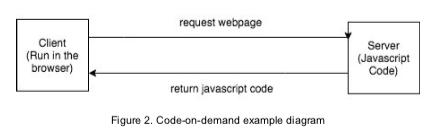
\includegraphics[width=0.4\textwidth]{./mobile-code1}
    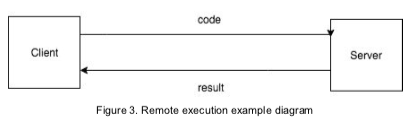
\includegraphics[width=0.4\textwidth]{./mobile-code2}
    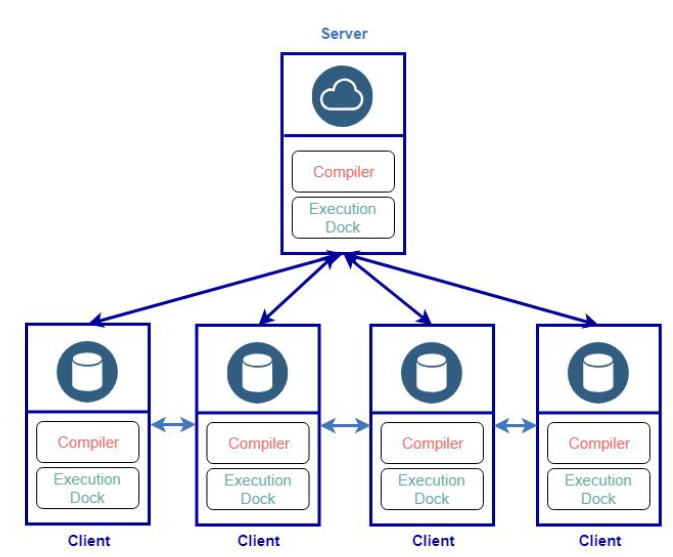
\includegraphics[width=0.4\textwidth]{./mobile-code3}
\end{center}
